\documentclass{beamer}
\usefonttheme[onlymath]{serif}
\usepackage[T1]{fontenc}
\usepackage[utf8]{inputenc}
\usepackage[english, icelandic]{babel}
\usepackage{amsmath}
\usepackage{amssymb}
\usepackage{amsthm}
\usepackage{gensymb}
\usepackage{parskip}
\usepackage{mathtools}
\usepackage{listings}
\usepackage{hyperref}
\usepackage{graphicx}
\usepackage{color}
\usepackage{enumerate}
\usepackage{tikz}
\usetikzlibrary{calc}
\usetikzlibrary{positioning}
\usetikzlibrary{angles}
\usetikzlibrary{shapes}
\usetikzlibrary{arrows}
\usepackage{verbatim}
\usepackage{multicol}
\usepackage{array}
\usepackage{minted}
\parskip 0pt


\DeclareMathOperator{\lcm}{lcm}
\newcommand\floor[1]{\left\lfloor#1\right\rfloor}
\newcommand\ceil[1]{\left\lceil#1\right\rceil}
\newcommand\abs[1]{\left|#1\right|}
\newcommand\p[1]{\left(#1\right)}
\newcommand\sqp[1]{\left[#1\right]}
\newcommand\cp[1]{\left\{#1\right\}}
\newcommand\norm[1]{\left\lVert#1\right\rVert}
\renewcommand\Im{\operatorname{Im}}
\renewcommand\Re{\operatorname{Re}}

\usetheme{metropolis}
\definecolor{dark yellow}{rgb} {0.6,0.6,0.0}
\definecolor{dark green}{rgb} {0.0,0.6,0.0}

\graphicspath{{myndir/}}

\usepackage{tikz}
\usetikzlibrary{arrows,shapes}
\usepackage{forest}

\title{Strings}
\author{Arnar Bjarni Arnarson \and Atli FF}
\institute{\href{http://ru.is/td}{School of Computer Science} \\[2pt] \href{http://ru.is}{Reykjavík University}}
\titlegraphic{\hfill
\includegraphics[height=0.6cm]{../../shared/kattis}}

\begin{document}
\maketitle

\begin{frame}[plain]{Today we're going to cover}
    \begin{itemize}
        \item String matching
        \begin{itemize}
            \item Naive algorithm
            \item Knuth--Morris--Pratt (KMP) algorithm
        \end{itemize}
        \item Tries
        \item Aho-Corasick
        \item Suffix Tries
        \item Suffix Arrays
    \end{itemize}
\end{frame}

\begin{frame}[plain]{String problems}
    \begin{itemize}
        \item Strings frequently appear in our kind of problems
        \begin{itemize}
            \item I/O
            \item Parsing
            \item Identifiers/names
            \item Data
        \end{itemize}
        \vspace{5pt}
        \item But sometimes strings play the key role
        \begin{itemize}
            \item We want to find properties of some given strings
            \item Is the string a palindrome?
        \end{itemize}
        \vspace{5pt}
        \item Here we're going to talk about things related to the latter type of problems
        \vspace{5pt}
        \item These problems can be hard, because the length of the strings are often huge
    \end{itemize}
\end{frame}

\begin{frame}[plain]{String matching}
	\begin{itemize}
		\item Given a string $S$ of length $n$,
		\item and a string $T$ of length $m$,
		\item find all occurrences of $T$ in $S$
    \end{itemize}
    \begin{itemize}
		\item Note:
        \begin{itemize}
            \item Occurrences may overlap
            \item Assume strings contain characters from some alphabet $\Sigma$
        \end{itemize}
	\end{itemize}
\end{frame}

\begin{frame}[plain]{String matching}
	Example:
	\begin{itemize}
		\item $S = \mathrm{cabcababacaba}$
		\item $T = \mathrm{aba}$
	\end{itemize}
    \begin{itemize}
        \item<2-> Three occurrences:
            \begin{itemize}
                \item<3-> $\mathrm{cabc{\color{red}{aba}}bacaba}$
                \item<4-> $\mathrm{cabcab{\color{red}{aba}}caba}$
                \item<5-> $\mathrm{cabcababac{\color{red}{aba}}}$
            \end{itemize}
    \end{itemize}
\end{frame}

\begin{frame}[plain]{Naive string matching algorithm}
	\begin{itemize}
	\item For each substring of length $m$ in $S$,
	\item check if that substring is equal to $T$.
	\end{itemize}
		
\end{frame}


\begin{frame}[plain]{Naive string matching algorithm}
    \begin{itemize}
        \item $S$: \texttt{\textcolor{red}{b}acbababaabcbab}
        \item $T$: \phantom{\texttt{}}\texttt{\textcolor{red}{a}babaca}
    \end{itemize}
\end{frame}
\begin{frame}[plain]{Naive string matching algorithm}
    \begin{itemize}
        \item $S$: \texttt{b\textcolor{green}{a}\textcolor{red}{c}bababaabcbab}
        \item $T$: \phantom{\texttt{a}}\texttt{\textcolor{green}{a}\textcolor{red}{b}abaca}
    \end{itemize}
\end{frame}
\begin{frame}[plain]{Naive string matching algorithm}
    \begin{itemize}
        \item $S$: \texttt{ba\textcolor{red}{c}bababaabcbab}
        \item $T$: \phantom{\texttt{aa}}\texttt{\textcolor{red}{a}babaca}
    \end{itemize}
\end{frame}
\begin{frame}[plain]{Naive string matching algorithm}
    \begin{itemize}
        \item $S$: \texttt{bac\textcolor{red}{b}ababaabcbab}
        \item $T$: \phantom{\texttt{aaa}}\texttt{\textcolor{red}{a}babaca}
    \end{itemize}
\end{frame}
\begin{frame}[plain]{Naive string matching algorithm}
    \begin{itemize}
        \item $S$: \texttt{bacb\textcolor{green}{ababa}\textcolor{red}{a}bcbab}
        \item $T$: \phantom{\texttt{aaaa}}\texttt{\textcolor{green}{ababa}\textcolor{red}{c}a}
    \end{itemize}
\end{frame}
\begin{frame}[plain]{Naive string matching algorithm}
    \begin{itemize}
        \item $S$: \texttt{bacba\textcolor{red}{b}abaabcbab}
        \item $T$: \phantom{\texttt{aaaaa}}\texttt{\textcolor{red}{a}babaca}
    \end{itemize}
\end{frame}
\begin{frame}[plain]{Naive string matching algorithm}
    \begin{itemize}
        \item $S$: \texttt{bacbab\textcolor{green}{aba}\textcolor{red}{a}bcbab}
        \item $T$: \phantom{\texttt{aaaaaa}}\texttt{\textcolor{green}{aba}\textcolor{red}{b}aca}
    \end{itemize}
\end{frame}
\begin{frame}[plain]{Naive string matching algorithm}
    \begin{itemize}
        \item $S$: \texttt{bacbaba\textcolor{red}{b}aabcbab}
        \item $T$: \phantom{\texttt{aaaaaaa}}\texttt{\textcolor{red}{a}babaca}
    \end{itemize}
\end{frame}
\begin{frame}[plain]{Naive string matching algorithm}
    \begin{itemize}
        \item $S$: \texttt{bacbabab\textcolor{green}{a}\textcolor{red}{a}bcbab}
        \item $T$: \phantom{\texttt{aaaaaaaa}}\texttt{\textcolor{green}{a}\textcolor{red}{b}abaca}
    \end{itemize}
    % \item<2-> $T$ is always shifted one forward
\end{frame}

\begin{frame}[plain,fragile]{Naive string matching algorithm}
    \begin{minted}[fontsize=\footnotesize]{cpp}
int string_match(const string &s, const string &t) {
    int n = s.size(),
        m = t.size();

    for (int i = 0; i + m - 1 < n; i++) {
        bool found = true;
        for (int j = 0; j < m; j++) {
            if (s[i + j] != t[j]) {
                found = false;
                break;
            }
        }
        if (found) {
            return i;
        }
    }

    return -1;
}
    \end{minted}
\end{frame}

\begin{frame}[plain]{Naive string matching algorithm}
    \begin{itemize}
        \item Double for-loop
            \begin{itemize}
                \item outer loop is $O(n)$ iterations
                \item inner loop is $O(m)$ iterations worst case
            \end{itemize}
        \item Time complexity is $O(nm)$ worst case
        \item<2-> Can we do better?
    \end{itemize}
\end{frame}

\begin{frame}[plain]
    \frametitle{Knuth--Morris--Pratt algorithm}
    \begin{itemize}
    \item The KMP algorithm avoids useless comparisons:
        \begin{itemize}
            \item $S$: \texttt{\textcolor{red}{b}acbababaabcbab}
            \item $T$: \phantom{\texttt{}}\texttt{\textcolor{red}{a}babaca}
        \end{itemize}
    \item[] \phantom{The number of shifts depend on which characters are currently matched}
    \end{itemize}
\end{frame}
\begin{frame}[plain]
    \frametitle{Knuth--Morris--Pratt algorithm}
    \begin{itemize}
    \item The KMP algorithm avoids useless comparisons:
        \begin{itemize}
            \item $S$: \texttt{b\textcolor{green}{a}\textcolor{red}{c}bababaabcbab}
            \item $T$: \phantom{\texttt{a}}\texttt{\textcolor{green}{a}\textcolor{red}{b}abaca}
        \end{itemize}
    \item[] \phantom{The number of shifts depend on which characters are currently matched}
    \end{itemize}
\end{frame}
\begin{frame}[plain]
    \frametitle{Knuth--Morris--Pratt algorithm}
    \begin{itemize}
    \item The KMP algorithm avoids useless comparisons:
        \begin{itemize}
            \item $S$: \texttt{ba\textcolor{red}{c}bababaabcbab}
            \item $T$: \phantom{\texttt{aa}}\texttt{\textcolor{red}{a}babaca}
        \end{itemize}
    \item[] \phantom{The number of shifts depend on which characters are currently matched}
    \end{itemize}
\end{frame}
\begin{frame}[plain]
    \frametitle{Knuth--Morris--Pratt algorithm}
    \begin{itemize}
    \item The KMP algorithm avoids useless comparisons:
        \begin{itemize}
            \item $S$: \texttt{bac\textcolor{red}{b}ababaabcbab}
            \item $T$: \phantom{\texttt{aaa}}\texttt{\textcolor{red}{a}babaca}
        \end{itemize}
    \item[] \phantom{The number of shifts depend on which characters are currently matched}
    \end{itemize}
\end{frame}
\begin{frame}[plain]
    \frametitle{Knuth--Morris--Pratt algorithm}
    \begin{itemize}
    \item The KMP algorithm avoids useless comparisons:
        \begin{itemize}
            \item $S$: \texttt{bacb\textcolor{green}{ababa}\textcolor{red}{a}bcbab}
            \item $T$: \phantom{\texttt{aaaa}}\texttt{\textcolor{green}{ababa}\textcolor{red}{c}a}
        \end{itemize}
    \item[] \phantom{The number of shifts depend on which characters are currently matched}
    \end{itemize}
\end{frame}
\begin{frame}[plain]
    \frametitle{Knuth--Morris--Pratt algorithm}
    \begin{itemize}
    \item The KMP algorithm avoids useless comparisons:
        \begin{itemize}
            \item $S$: \texttt{bacbab\textcolor{green}{aba}\textcolor{red}{a}bcbab}
            \item $T$: \phantom{\texttt{aaaaaa}}\texttt{\textcolor{green}{aba}\textcolor{red}{b}aca}
        \end{itemize}
    \item[] \phantom{The number of shifts depend on which characters are currently matched}
    \end{itemize}
\end{frame}
\begin{frame}[plain]
    \frametitle{Knuth--Morris--Pratt algorithm}
    \begin{itemize}
    \item The KMP algorithm avoids useless comparisons:
        \begin{itemize}
            \item $S$: \texttt{bacbabab\textcolor{green}{a}\textcolor{red}{a}bcbab}
            \item $T$: \phantom{\texttt{aaaaaaaa}}\texttt{\textcolor{green}{a}\textcolor{red}{b}abaca}
        \end{itemize}
    \item<2-> The number of shifts depend on which characters are currently matched
    \end{itemize}
\end{frame}

\begin{frame}[plain]
    \frametitle{Knuth--Morris--Pratt algorithm}
    \begin{itemize}
        \item How are the number of shifts determined?
            \vspace{5pt}
        \item Let {\footnotesize $\pi[q] = \max \{ k : k < q \textrm{ and } T[1\ldots k] \textrm{ is a suffix of } T[1\ldots q] \}$}
            \vspace{5pt}
        \item<2-> Example:\\
            \begin{center}
                % \hspace{-50px}
                \begin{tabular}{cccccccc}
                    $i$ & $1$ & $2$ & $3$ & $4$ & $5$ & $6$ & $7$ \\
                    \hline
                    $T[i]$&\texttt{a}&\texttt{b}&\texttt{a}&\texttt{b}&\texttt{a}&\texttt{c}&\texttt{a} \\
                    $\pi[i]$ & $0$ & $0$ & $1$ & $2$ & $3$ & $0$ & $1$\\
                \end{tabular}
            \end{center}
    \vspace{5pt}
        \item<3-> If, at position $i$, $q$ characters match (i.e. $T[1\ldots q] = S[i\ldots i+q-1]$), then
            \begin{itemize}
                \item if $q = 0$, shift pattern $1$ position right
                \item otherwise, shift pattern $q - \pi[q]$ positions right
            \end{itemize}
    \end{itemize}
\end{frame}

\begin{frame}[plain]
    \frametitle{Knuth--Morris--Pratt algorithm}
    \begin{itemize}
        \item Example:
        \begin{itemize}
            \item $S$: \texttt{bacb\textcolor{green}{ababa}\textcolor{red}{a}bcbab}
            \item $T$: \phantom{\texttt{aaaa}}\texttt{\textcolor{green}{ababa}\textcolor{red}{c}a}
            \item<2-> $5$ characters match, so $q = 5$
            \item<3-> $\pi[q] = \pi[5] = 3$
            \item<4-> Then shift $q - \pi[q] = 5 - 3 = 2$ positions
            \item<5-> $S$: \texttt{bacbab\textcolor{green}{aba}\textcolor{red}{a}bcbab}
            \item<5-> $T$: \phantom{\texttt{aaaaaa}}\texttt{\textcolor{green}{aba}\textcolor{red}{b}aca}
        \end{itemize}
    \end{itemize}
\end{frame}

\begin{frame}[plain]
    \frametitle{Knuth--Morris--Pratt algorithm}
    \begin{itemize}
        \item Given $\pi$, matching only takes $O(n)$ time
        \item $\pi$ can be computed in $O(m)$ time
        \item Total time complexity of KMP therefore $O(n+m)$ worst case
    \end{itemize}
\end{frame}

\begin{frame}[plain,fragile]{Knuth--Morris--Pratt algorithm}
    \begin{minted}[fontsize=\scriptsize]{cpp}
vi kmppi(string &p) {
  int m = p.size(), i = 0, j = -1; 
  vi b(m + 1, -1);
  while(i < m) { 
    while(j >= 0 && p[i] != p[j]) j = b[j]; 
    b[++i] = ++j; 
  } 
  return b; 
}

vi kmp(string &s, string &p) {
  int n = s.size(), m = p.size(), i = 0, j = 0;
  vi b = kmppi(p), a = vi(); 
  while(i < n) {
    while(j >= 0 && s[i] != p[j]) j = b[j];
    ++i; ++j; 
    if(j == m) { 
      a.push_back(i - j);
      j = b[j]; 
    } 
  } 
  return a; }
    \end{minted}
\end{frame}

\begin{frame}[plain]{Sets of strings}
    \begin{itemize}
\item We often have sets (or maps) of strings
\item Insertions and lookups usually guarantee $O(\log n)$ comparisons
    \vspace{10pt}
\item But string comparisons are actually pretty expensive...
    \vspace{10pt}
\item There are other data structures, like tries, which do this in a more clever way
    \end{itemize}
\end{frame}

\begin{frame}[plain]{Tries}
	\begin{itemize}
        \item Tries contain strings not at every node, but as paths in a tree.
        \item Each node only has a character and we say the trie contains the string if you can get it by walking along nodes starting at the root.
        \item The nodes can also carry additional data, quite a lot in fact, as we will see later.
    \end{itemize}
\end{frame}

\begin{frame}[plain]{Example}
	\begin{tikzpicture}
		\node[draw, circle, thick, white] (0) at (-1, 0) {};
		\node[draw, circle, thick, inner sep = 1.0pt] (1) at (0, 0) {};
		\node[draw, circle, thick, inner sep = 1.0pt] (2) at (1, 1) {};
		\node[draw, circle, thick, inner sep = 1.0pt] (3) at (1, 0) {};
		\node[draw, circle, thick, inner sep = 1.0pt] (4) at (1, -1) {};
		\node[draw, circle, thick, inner sep = 1.0pt] (5) at (2, 0) {};
		\node[draw, circle, thick, inner sep = 1.0pt] (6) at (3, 0) {};
		\node[draw, circle, thick, inner sep = 1.0pt] (7) at (4, 0) {};
		\node[draw, circle, thick, inner sep = 1.0pt] (8) at (5, 0) {};
		\node[draw, circle, thick, inner sep = 1.0pt] (9) at (6, 0) {};
		\node[draw, circle, thick, inner sep = 1.0pt] (10) at (2, -1) {};
		\node[draw, circle, thick, inner sep = 1.0pt] (11) at (3, -1) {};
		\node[draw, circle, thick, inner sep = 1.0pt] (12) at (4, -1) {};
		\node[draw, circle, thick, inner sep = 1.0pt] (13) at (2, 1) {};
		\node[draw, circle, thick, inner sep = 1.0pt] (14) at (3, 1) {};
		\node[draw, circle, thick, inner sep = 1.0pt] (15) at (4, 1) {};
		\node[draw, circle, thick, inner sep = 1.0pt] (16) at (5, 1) {};
		\node[draw, circle, thick, inner sep = 1.0pt] (17) at (6, 1) {};
		\node[draw, circle, thick, inner sep = 1.0pt] (18) at (5, -1) {};
		\node[draw, circle, thick, inner sep = 1.0pt] (19) at (6, -1) {};
		\node[draw, circle, thick, inner sep = 1.0pt] (20) at (7, -1) {};

		\path[draw, thick, ->] (0) -- (1);
		\path[draw, thick] (1) -- (2);
		\path[draw, thick] (1) -- (3);
		\path[draw, thick] (3) -- (5);
		\path[draw, thick] (5) -- (6);
		\path[draw, thick] (6) -- (7);
		\path[draw, thick] (7) -- (8);
		\path[draw, thick] (8) -- (9);
		\path[draw, thick] (1) -- (4);
		\path[draw, thick] (4) -- (10);
		\path[draw, thick] (10) -- (11);
		\path[draw, thick] (11) -- (12);
		\path[draw, thick] (2) -- (13);
		\path[draw, thick] (13) -- (14);
		\path[draw, thick] (14) -- (15);
		\path[draw, thick] (15) -- (16);
		\path[draw, thick] (16) -- (17);
		\path[draw, thick] (7) -- (18);
		\path[draw, thick] (18) -- (19);
		\path[draw, thick] (19) -- (20);

		\node at (0.5, 0.2) {b};
		\node at (1.5, 0.2) {e};
		\node at (2.5, 0.2) {r};
		\node at (3.5, 0.2) {g};
		\node at (4.5, 0.2) {u};
		\node at (5.5, 0.2) {r};
		\node at (0.6, -0.4) {n};
		\node at (1.5, -0.8) {a};
		\node at (2.5, -0.8) {l};
		\node at (3.5, -0.8) {a};
		\node at (0.5, 0.8) {s};
		\node at (1.5, 1.2) {a};
		\node at (2.5, 1.2) {n};
		\node at (3.5, 1.2) {d};
		\node at (4.5, 1.2) {r};
		\node at (5.5, 1.2) {a};
		\node at (4.7, -0.4) {þ};
		\node at (5.5, -0.8) {ó};
		\node at (6.5, -0.8) {r};
		%\only<all:2-3> { \node at (6,3) {$v$}; }
		%\only<all:3> { \node at (5,1) {$x$}; }
    \end{tikzpicture}
	\begin{itemize}
        \item Examples of strings in this trie include:
		\begin{itemize}
			\item<3-> ,,sandra'',
			\item<4-> ,,nala'',
			\item<5-> ,,bergur'',
			\item<6-> ,,bergþór'',
			\item<7-> ,,san'' and
			\item<8-> ,,'' (empty string)
        \end{itemize}
    \end{itemize}
\end{frame}

\begin{frame}[plain]{End nodes}
	\begin{itemize}
        \item It is common to mark some nodes as end nodes.
        \item This is an example of extra data to put into nodes.
        \item Then we can consider a string $s$ to be in the tree if you can walk through the tree to get the string \textbf{and} end at an end node.
    \end{itemize}
\end{frame}

\begin{frame}[plain]{Example}
	\begin{tikzpicture}
		\node[draw, circle, thick, white] (0) at (-1, 0) {};
		\node[draw, circle, thick, inner sep = 1.0pt] (1) at (0, 0) {};
		\node[draw, circle, thick, inner sep = 1.0pt] (2) at (1, 1) {};
		\node[draw, circle, thick, inner sep = 1.0pt] (3) at (1, 0) {};
		\node[draw, circle, thick, fill, inner sep = 1.0pt] (4) at (1, -1) {};
		\node[draw, circle, thick, inner sep = 1.0pt] (5) at (2, 0) {};
		\node[draw, circle, thick, inner sep = 1.0pt] (6) at (3, 0) {};
		\node[draw, circle, thick, inner sep = 1.0pt] (7) at (4, 0) {};
		\node[draw, circle, thick, inner sep = 1.0pt] (8) at (5, 0) {};
		\node[draw, circle, thick, fill, inner sep = 1.0pt] (9) at (6, 0) {};
		\node[draw, circle, thick, inner sep = 1.0pt] (10) at (2, -1) {};
		\node[draw, circle, thick, inner sep = 1.0pt] (11) at (3, -1) {};
		\node[draw, circle, thick, fill, inner sep = 1.0pt] (12) at (4, -1) {};
		\node[draw, circle, thick, inner sep = 1.0pt] (13) at (2, 1) {};
		\node[draw, circle, thick, inner sep = 1.0pt] (14) at (3, 1) {};
		\node[draw, circle, thick, inner sep = 1.0pt] (15) at (4, 1) {};
		\node[draw, circle, thick, inner sep = 1.0pt] (16) at (5, 1) {};
		\node[draw, circle, thick, fill, inner sep = 1.0pt] (17) at (6, 1) {};
		\node[draw, circle, thick, inner sep = 1.0pt] (18) at (5, -1) {};
		\node[draw, circle, thick, inner sep = 1.0pt] (19) at (6, -1) {};
		\node[draw, circle, thick, fill, inner sep = 1.0pt] (20) at (7, -1) {};

		\path[draw, thick, ->] (0) -- (1);
		\path[draw, thick] (1) -- (2);
		\path[draw, thick] (1) -- (3);
		\path[draw, thick] (3) -- (5);
		\path[draw, thick] (5) -- (6);
		\path[draw, thick] (6) -- (7);
		\path[draw, thick] (7) -- (8);
		\path[draw, thick] (8) -- (9);
		\path[draw, thick] (1) -- (4);
		\path[draw, thick] (4) -- (10);
		\path[draw, thick] (10) -- (11);
		\path[draw, thick] (11) -- (12);
		\path[draw, thick] (2) -- (13);
		\path[draw, thick] (13) -- (14);
		\path[draw, thick] (14) -- (15);
		\path[draw, thick] (15) -- (16);
		\path[draw, thick] (16) -- (17);
		\path[draw, thick] (7) -- (18);
		\path[draw, thick] (18) -- (19);
		\path[draw, thick] (19) -- (20);

		\node at (0.5, 0.2) {b};
		\node at (1.5, 0.2) {e};
		\node at (2.5, 0.2) {r};
		\node at (3.5, 0.2) {g};
		\node at (4.5, 0.2) {u};
		\node at (5.5, 0.2) {r};
		\node at (0.6, -0.4) {n};
		\node at (1.5, -0.8) {a};
		\node at (2.5, -0.8) {l};
		\node at (3.5, -0.8) {a};
		\node at (0.5, 0.8) {s};
		\node at (1.5, 1.2) {a};
		\node at (2.5, 1.2) {n};
		\node at (3.5, 1.2) {d};
		\node at (4.5, 1.2) {r};
		\node at (5.5, 1.2) {a};
		\node at (4.7, -0.4) {þ};
		\node at (5.5, -0.8) {ó};
		\node at (6.5, -0.8) {r};
		%\only<all:2-3> { \node at (6,3) {$v$}; }
		%\only<all:3> { \node at (5,1) {$x$}; }
    \end{tikzpicture}
	\begin{itemize}
		\item<2-> The strings in the trie are:
		\begin{itemize}
			\item<3-> ,,sandra'',
			\item<4-> ,,nala'',
			\item<5-> ,,bergur'',
			\item<6-> ,,bergþór'' and
			\item<7-> ,,n''
        \end{itemize}
    \end{itemize}
\end{frame}

\begin{frame}[plain]{Adding strings}
    \begin{itemize}
        \item What if we want to add a string to a trie?
        \item We walk through it as usual, but simply add nodes when we find ourself at a dead end with letters left to walk through.
        \item This increases the size of the tree by at most the size of the string.
    \end{itemize}
\end{frame}

\begin{frame}[plain]{Example}
	\begin{tikzpicture}
		\node[draw, circle, white, thick, inner sep = 1.0pt] at (4, -2) {}; %alignment

		\node[draw, circle, thick, white] (0) at (-1, 0) {};
		\only<all:1-2, 4-8, 10-15, 17-27, 29-36, 38-46, 48-61, 63-> { \node[draw, circle, thick, inner sep = 1.0pt] (1) at (0, 0) {}; }
		\only<all:3, 9, 16, 28, 37, 47, 62> { \node[draw, circle, blue, thick, inner sep = 1.0pt] (1) at (0, 0) {}; }

		\only<all:5-9, 11-16, 18-28, 30-37, 39-47, 49-62, 64-> { \node[draw, circle, thick, inner sep = 1.0pt] (2) at (1, 0) {}; }
		\only<all:4, 10, 17, 29, 38, 48, 63> { \node[draw, circle, blue, thick, inner sep = 1.0pt] (2) at (1, 0) {}; }

		\only<all:6-10, 12-17, 19-38, 40-> { \node[draw, circle, thick, inner sep = 1.0pt] (3) at (2, 0) {}; }
		\only<all:5, 11, 18, 39> { \node[draw, circle, blue, thick, inner sep = 1.0pt] (3) at (2, 0) {}; }

		\only<all:7-> { \node[draw, circle, fill, thick, inner sep = 1.0pt] (4) at (3, 0) {}; }
		\only<all:6> { \node[draw, circle, blue, thick, inner sep = 1.0pt] (4) at (3, 0) {}; }

		\only<all:13-18, 20-39, 41-> { \node[draw, circle, thick, inner sep = 1.0pt] (5) at (3, -1) {}; }
		\only<all:12, 19, 40> { \node[draw, circle, blue, thick, inner sep = 1.0pt] (5) at (3, -1) {}; }

		\only<all:14-> { \node[draw, circle, fill, thick, inner sep = 1.0pt] (6) at (4, -1) {}; }
		\only<all:13> { \node[draw, circle, blue, thick, inner sep = 1.0pt] (6) at (4, -1) {}; }

		\only<all:21-> { \node[draw, circle, thick, inner sep = 1.0pt] (7) at (4, -2) {}; }
		\only<all:20> { \node[draw, circle, blue, thick, inner sep = 1.0pt] (7) at (4, -2) {}; }

		\only<all:22-> { \node[draw, circle, thick, inner sep = 1.0pt] (8) at (5, -2) {}; }
		\only<all:21> { \node[draw, circle, blue, thick, inner sep = 1.0pt] (8) at (5, -2) {}; }

		\only<all:23-> { \node[draw, circle, thick, inner sep = 1.0pt] (9) at (6, -2) {}; }
		\only<all:22> { \node[draw, circle, blue, thick, inner sep = 1.0pt] (9) at (6, -2) {}; }

		\only<all:24-> { \node[draw, circle, thick, inner sep = 1.0pt] (10) at (7, -2) {}; }
		\only<all:23> { \node[draw, circle, blue, thick, inner sep = 1.0pt] (10) at (7, -2) {}; }

		\only<all:25-> { \node[draw, circle, thick, inner sep = 1.0pt] (11) at (8, -2) {}; }
		\only<all:24> { \node[draw, circle, blue, thick, inner sep = 1.0pt] (11) at (8, -2) {}; }

		\only<all:26-> { \node[draw, circle, fill, thick, inner sep = 1.0pt] (12) at (9, -2) {}; }
		\only<all:25> { \node[draw, circle, blue, thick, inner sep = 1.0pt] (12) at (9, -2) {}; }

		\only<all:31-48, 50-63, 65-> { \node[draw, circle, thick, inner sep = 1.0pt] (13) at (2, 1) {}; }
		\only<all:30, 49, 64> { \node[draw, circle, blue, thick, inner sep = 1.0pt] (13) at (2, 1) {}; }

		\only<all:32-49, 51-64, 66-> { \node[draw, circle, thick, inner sep = 1.0pt] (14) at (3, 1) {}; }
		\only<all:31, 50, 65> { \node[draw, circle, blue, thick, inner sep = 1.0pt] (14) at (3, 1) {}; }

		\only<all:33-50, 52-65, 67-> { \node[draw, circle, thick, inner sep = 1.0pt] (15) at (4, 1) {}; }
		\only<all:32, 51, 66> { \node[draw, circle, blue, thick, inner sep = 1.0pt] (15) at (4, 1) {}; }

		\only<all:34-51, 53-66, 68-> { \node[draw, circle, thick, inner sep = 1.0pt] (16) at (5, 1) {}; }
		\only<all:33, 52, 67> { \node[draw, circle, blue, thick, inner sep = 1.0pt] (16) at (5, 1) {}; }

		\only<all:35-52, 54-67, 69-> { \node[draw, circle, fill, thick, inner sep = 1.0pt] (17) at (6, 1) {}; }
		\only<all:34, 53, 68> { \node[draw, circle, blue, thick, inner sep = 1.0pt] (17) at (6, 1) {}; }

		\only<all:42-> { \node[draw, circle, thick, inner sep = 1.0pt] (18) at (4, 0) {}; }
		\only<all:41> { \node[draw, circle, blue, thick, inner sep = 1.0pt] (18) at (4, 0) {}; }

		\only<all:43-> { \node[draw, circle, thick, inner sep = 1.0pt] (19) at (5, 0) {}; }
		\only<all:42> { \node[draw, circle, blue, thick, inner sep = 1.0pt] (19) at (5, 0) {}; }

		\only<all:44-> { \node[draw, circle, thick, inner sep = 1.0pt] (20) at (6, 0) {}; }
		\only<all:43> { \node[draw, circle, blue, thick, inner sep = 1.0pt] (20) at (6, 0) {}; }

		\only<all:45-> { \node[draw, circle, fill, thick, inner sep = 1.0pt] (21) at (7, 0) {}; }
		\only<all:44> { \node[draw, circle, blue, thick, inner sep = 1.0pt] (21) at (7, 0) {}; }

		\only<all:55-68, 70-> { \node[draw, circle, thick, inner sep = 1.0pt] (22) at (7, 1) {}; }
		\only<all:54, 69> { \node[draw, circle, blue, thick, inner sep = 1.0pt] (22) at (7, 1) {}; }

		\only<all:56-> { \node[draw, circle, thick, inner sep = 1.0pt] (23) at (8, 1) {}; }
		\only<all:55> { \node[draw, circle, blue, thick, inner sep = 1.0pt] (23) at (8, 1) {}; }

		\only<all:57-> { \node[draw, circle, thick, inner sep = 1.0pt] (24) at (8, 0) {}; }
		\only<all:56> { \node[draw, circle, blue, thick, inner sep = 1.0pt] (24) at (8, 0) {}; }

		\only<all:58-> { \node[draw, circle, thick, inner sep = 1.0pt] (25) at (9, 0) {}; }
		\only<all:57> { \node[draw, circle, blue, thick, inner sep = 1.0pt] (25) at (9, 0) {}; }

		\only<all:59-> { \node[draw, circle, thick, inner sep = 1.0pt] (26) at (9, 1) {}; }
		\only<all:58> { \node[draw, circle, blue, thick, inner sep = 1.0pt] (26) at (9, 1) {}; }

		\only<all:1-> { \node[draw, circle, white, thick, inner sep = 1.0pt] (27) at (10, 1) {}; } %alignment
		\only<all:60-> { \node[draw, circle, fill, thick, inner sep = 1.0pt] (27) at (10, 1) {}; }
		\only<all:59> { \node[draw, circle, blue, thick, inner sep = 1.0pt] (27) at (10, 1) {}; }

		\only<all:71-> { \node[draw, circle, thick, inner sep = 1.0pt] (28) at (7, 2) {}; }
		\only<all:70> { \node[draw, circle, blue, thick, inner sep = 1.0pt] (28) at (7, 2) {}; }

		\only<all:72-> { \node[draw, circle, thick, inner sep = 1.0pt] (29) at (6, 2) {}; }
		\only<all:71> { \node[draw, circle, blue, thick, inner sep = 1.0pt] (29) at (6, 2) {}; }

		\only<all:73-> { \node[draw, circle, thick, inner sep = 1.0pt] (30) at (5, 2) {}; }
		\only<all:72> { \node[draw, circle, blue, thick, inner sep = 1.0pt] (30) at (5, 2) {}; }

		\only<all:74-> { \node[draw, circle, thick, inner sep = 1.0pt] (31) at (4, 2) {}; }
		\only<all:73> { \node[draw, circle, blue, thick, inner sep = 1.0pt] (31) at (4, 2) {}; }

		\only<all:75-> { \node[draw, circle, fill, thick, inner sep = 1.0pt] (32) at (3, 2) {}; }
		\only<all:74> { \node[draw, circle, blue, thick, inner sep = 1.0pt] (32) at (3, 2) {}; }


		\path[draw, thick, ->] (0) -- (1);
		\only<all:4-> { \path[draw, thick] (1) -- (2); }
		\only<all:5-> { \path[draw, thick] (2) -- (3); }
		\only<all:6-> { \path[draw, thick] (3) -- (4); }
		\only<all:12-> { \path[draw, thick] (3) -- (5); }
		\only<all:13-> { \path[draw, thick] (5) -- (6); }
		\only<all:20-> { \path[draw, thick] (5) -- (7); }
		\only<all:21-> { \path[draw, thick] (7) -- (8); }
		\only<all:22-> { \path[draw, thick] (8) -- (9); }
		\only<all:23-> { \path[draw, thick] (9) -- (10); }
		\only<all:24-> { \path[draw, thick] (10) -- (11); }
		\only<all:25-> { \path[draw, thick] (11) -- (12); }
		\only<all:30-> { \path[draw, thick] (2) -- (13); }
		\only<all:31-> { \path[draw, thick] (13) -- (14); }
		\only<all:32-> { \path[draw, thick] (14) -- (15); }
		\only<all:33-> { \path[draw, thick] (15) -- (16); }
		\only<all:34-> { \path[draw, thick] (16) -- (17); }
		\only<all:41-> { \path[draw, thick] (5) -- (18); }
		\only<all:42-> { \path[draw, thick] (18) -- (19); }
		\only<all:43-> { \path[draw, thick] (19) -- (20); }
		\only<all:44-> { \path[draw, thick] (20) -- (21); }
		\only<all:54-> { \path[draw, thick] (17) -- (22); }
		\only<all:55-> { \path[draw, thick] (22) -- (23); }
		\only<all:56-> { \path[draw, thick] (23) -- (24); }
		\only<all:57-> { \path[draw, thick] (24) -- (25); }
		\only<all:58-> { \path[draw, thick] (25) -- (26); }
		\only<all:59-> { \path[draw, thick] (26) -- (27); }
		\only<all:70-> { \path[draw, thick] (22) -- (28); }
		\only<all:71-> { \path[draw, thick] (28) -- (29); }
		\only<all:72-> { \path[draw, thick] (29) -- (30); }
		\only<all:73-> { \path[draw, thick] (30) -- (31); }
		\only<all:74-> { \path[draw, thick] (31) -- (32); }

		%\only<all:1-> { \node[white] at (3.5, -0.8) {r}; } %alignment
		\only<all:4-> { \node at (0.5, 0.2) {a}; }
		\only<all:5-> { \node at (1.5, 0.2) {p}; }
		\only<all:6-> { \node at (2.5, 0.2) {i}; }
		\only<all:12-> { \node at (2.7, -0.5) {a}; }
		\only<all:13-> { \node at (3.5, -0.8) {r}; }
		\only<all:20-> { \node at (3.7, -1.4) {k}; }
		\only<all:21-> { \node at (4.5, -1.8) {ö}; }
		\only<all:22-> { \node at (5.5, -1.8) {t}; }
		\only<all:23-> { \node at (6.5, -1.8) {t}; }
		\only<all:24-> { \node at (7.5, -1.8) {u}; }
		\only<all:25-> { \node at (8.5, -1.8) {r}; }
		\only<all:30-> { \node at (1.5, 0.8) {l}; }
		\only<all:31-> { \node at (2.5, 1.2) {t}; }
		\only<all:32-> { \node at (3.5, 1.2) {a}; }
		\only<all:33-> { \node at (4.5, 1.2) {r}; }
		\only<all:34-> { \node at (5.5, 1.2) {i}; }
		\only<all:41-> { \node at (3.6, -0.2) {s}; }
		\only<all:42-> { \node at (4.5, 0.2) {p}; }
		\only<all:43-> { \node at (5.5, 0.2) {i}; }
		\only<all:44-> { \node at (6.5, 0.2) {l}; }
		\only<all:54-> { \node at (6.5, 1.2) {s}; }
		\only<all:55-> { \node at (7.5, 1.2) {t}; }
		\only<all:56-> { \node at (8.2, 0.5) {a}; }
		\only<all:57-> { \node at (8.5, 0.2) {f}; }
		\only<all:58-> { \node at (9.2, 0.5) {l}; }
		\only<all:59-> { \node at (9.5, 1.2) {a}; }
		\only<all:70-> { \node at (7.2, 1.7) {g}; }
		\only<all:71-> { \node at (6.5, 2.2) {a}; }
		\only<all:72-> { \node at (5.5, 2.2) {n}; }
		\only<all:73-> { \node at (4.5, 2.2) {g}; }
		\only<all:74-> { \node at (3.5, 2.2) {a}; }

		%\node at (6.5, -0.8) {r};
		\only<all:1-> { \node[white] at (6,3) {,,api''}; } %alignment
		\only<all:2-3> { \node at (6,3) {,,api''}; }
		\only<all:4> { \node at (6,3) {,,pi''}; }
		\only<all:5> { \node at (6,3) {,,i''}; }
		\only<all:6> { \node at (6,3) {,,''}; }
		\only<all:8-9> { \node at (6,3) {,,apar''}; }
		\only<all:10> { \node at (6,3) {,,par''}; }
		\only<all:11> { \node at (6,3) {,,ar''}; }
		\only<all:12> { \node at (6,3) {,,r''}; }
		\only<all:13> { \node at (6,3) {,,''}; }
		\only<all:15-16> { \node at (6,3) {,,apaköttur''}; }
		\only<all:17> { \node at (6,3) {,,paköttur''}; }
		\only<all:18> { \node at (6,3) {,,aköttur''}; }
		\only<all:19> { \node at (6,3) {,,köttur''}; }
		\only<all:20> { \node at (6,3) {,,öttur''}; }
		\only<all:21> { \node at (6,3) {,,ttur''}; }
		\only<all:22> { \node at (6,3) {,,tur''}; }
		\only<all:23> { \node at (6,3) {,,ur''}; }
		\only<all:24> { \node at (6,3) {,,r''}; }
		\only<all:25> { \node at (6,3) {,,''}; }
		\only<all:27-28> { \node at (6,3) {,,altari''}; }
		\only<all:29> { \node at (6,3) {,,ltari''}; }
		\only<all:30> { \node at (6,3) {,,tari''}; }
		\only<all:31> { \node at (6,3) {,,ari''}; }
		\only<all:32> { \node at (6,3) {,,ri''}; }
		\only<all:33> { \node at (6,3) {,,i''}; }
		\only<all:34> { \node at (6,3) {,,''}; }
		\only<all:36-37> { \node at (6,3) {,,apaspil''}; }
		\only<all:38> { \node at (6,3) {,,paspil''}; }
		\only<all:39> { \node at (6,3) {,,aspil''}; }
		\only<all:40> { \node at (6,3) {,,spil''}; }
		\only<all:41> { \node at (6,3) {,,pil''}; }
		\only<all:42> { \node at (6,3) {,,il''}; }
		\only<all:43> { \node at (6,3) {,,l''}; }
		\only<all:44> { \node at (6,3) {,,''}; }
		\only<all:46-47> { \node at (6,3) {,,altaristafla''}; }
		\only<all:48> { \node at (6,3) {,,ltaristafla''}; }
		\only<all:49> { \node at (6,3) {,,taristafla''}; }
		\only<all:50> { \node at (6,3) {,,aristafla''}; }
		\only<all:51> { \node at (6,3) {,,ristafla''}; }
		\only<all:52> { \node at (6,3) {,,istafla''}; }
		\only<all:53> { \node at (6,3) {,,stafla''}; }
		\only<all:54> { \node at (6,3) {,,tafla''}; }
		\only<all:55> { \node at (6,3) {,,afla''}; }
		\only<all:56> { \node at (6,3) {,,fla''}; }
		\only<all:57> { \node at (6,3) {,,la''}; }
		\only<all:58> { \node at (6,3) {,,a''}; }
		\only<all:59> { \node at (6,3) {,,''}; }
		\only<all:61-62> { \node at (6,3) {,,altarisganga''}; }
		\only<all:63> { \node at (6,3) {,,ltarisganga''}; }
		\only<all:64> { \node at (6,3) {,,tarisganga''}; }
		\only<all:65> { \node at (6,3) {,,arisganga''}; }
		\only<all:66> { \node at (6,3) {,,risganga''}; }
		\only<all:67> { \node at (6,3) {,,isganga''}; }
		\only<all:68> { \node at (6,3) {,,sganga''}; }
		\only<all:69> { \node at (6,3) {,,ganga''}; }
		\only<all:70> { \node at (6,3) {,,anga''}; }
		\only<all:71> { \node at (6,3) {,,nga''}; }
		\only<all:72> { \node at (6,3) {,,ga''}; }
		\only<all:73> { \node at (6,3) {,,a''}; }
		\only<all:74> { \node at (6,3) {,,''}; }
    \end{tikzpicture}
\end{frame}

\begin{frame}[plain,fragile]{Tries}
    \begin{minted}{cpp}
struct node {
    node* children[26];
    bool is_end;

    node() {
        memset(children, 0, sizeof(children));
        is_end = false;
    }
};
    \end{minted}
\end{frame}

\begin{frame}[plain,fragile]{Tries}
    \begin{minted}{cpp}
void insert(node* nd, char *s) {
    if (*s) {
        if (!nd->children[*s - 'a'])
            nd->children[*s - 'a'] = new node();

        insert(nd->children[*s - 'a'], s + 1);
    } else {
        nd->is_end = true;
    }
}
    \end{minted}
\end{frame}

\begin{frame}[plain,fragile]{Tries}
    \begin{minted}{cpp}
bool contains(node* nd, char *s) {
    if (*s) {
        if (!nd->children[*s - 'a'])
            return false;

        return contains(nd->children[*s - 'a'], s + 1);
    } else {
        return nd->is_end;
    }
}
    \end{minted}
\end{frame}

\begin{frame}[plain,fragile]{Tries}
    \begin{minted}{cpp}
node *trie = new node();

insert(trie, "banani");

if (contains(trie, "banani")) {
    // ...
}
    \end{minted}
\end{frame}

\begin{frame}[plain]{Tries}
    \begin{itemize}
        \item Time complexity?
        \vspace{10pt}
        \item Let $k$ be the length of the string we're inserting/looking for
        \item Lookup is $\mathcal{O}(k)$ and insertion is both $\mathcal{O}(k|\Sigma|)$
        \item The insertion takes this time because we might have to make $k$ nodes, each needing $|\Sigma|$ pointers initialized
    \end{itemize}
\end{frame}

\begin{frame}[plain]{Aho-Corasick}
	\begin{itemize}
        \item Let us now have some string $s$ and a list of $n$ strings $p$, where we denote the $j$-th string by $p_j$.
        \item Let $|s|$ be the length of $s$ and $|p| = |p_1| + \dots + |p_n|$.
        \item We want to find all substrings of $s$ that are in the list $p$.
        \item We could run KMP $n$ times, once for each $p_j$, for a time complexity of $\mathcal{O}(n \cdot |s| + |p|)$.
        \item The Aho-Corasick algorithm improves on this.
    \end{itemize}
\end{frame}

\begin{frame}[plain]{The algorithm}
	\begin{itemize}
        \item We start by putting all strings in $p$ into a trie $T$, we want to turn this into a finite state automata.
        \item We then want to turn $T$ into a finite state automata.
        \item The nodes of the trie will be our states but the transitions from each state will correspond to a letter from $\Sigma$.
    \end{itemize}
\end{frame}

\begin{frame}[plain]{The automata}
	\begin{itemize}
        \item Suppose we are in node $v$ in $T$ and want to transition according to the letter $c$ in $\Sigma$.
        \item If there is an node corresponding to adding a $c$ after $v$ we can travel there.
        \item If not we need to travel back to some node $w$ so the string corresponding to $w$ is a suffix of the one corresponding to $v$.
        \item We want to drop the least amount of information, so we want $w$ to be as long as possible.
        \item We call these transitions \emph{suffix links}. Note that they are essentially independent of $c$.
        \item We let the suffix link of the root point back to itself for simplicity's sake.
    \end{itemize}
\end{frame}

\begin{frame}[plain]{Suffix links}
	\begin{itemize}
        \item How do we find the suffix links?
        % \item We will cheat and borrow a method from the future, dynamic programming.
        \item Let $f(w, c)$ denote the transition from node $w$ with the letter $c$ and let $g(w)$ be the suffix link of $w$.
        \item Also let $p$ be the parent of $p$ and $f(p, a) = v$. Then $g(v) = f(g(p), a)$.
        \item Thus we have a recursive formula we can use.
    \end{itemize}
\end{frame}

\begin{frame}[plain]{Example}
	\begin{tikzpicture}
		\node[draw, circle, thick, white] (0) at (-1, 0) {};

		\only<all:2, 3> { \node[draw, circle, fill, blue, thick, inner sep = 1.0pt] at (2, -1) {}; }
		\only<all:4, 5> { \node[draw, circle, fill, blue, thick, inner sep = 1.0pt] at (3, -1) {}; }
		\only<all:6, 7> { \node[draw, circle, fill, blue, thick, inner sep = 1.0pt] at (4, -1) {}; }
		\only<all:8, 9> { \node[draw, circle, fill, blue, thick, inner sep = 1.0pt] at (2, 1) {}; }
		\only<all:10, 11> { \node[draw, circle, fill, blue, thick, inner sep = 1.0pt] at (3, 1) {}; }
		\only<all:12, 13> { \node[draw, circle, fill, blue, thick, inner sep = 1.0pt] at (4, 1) {}; }

		\node[draw, circle, thick, inner sep = 1.0pt] (1) at (0, 0) {};
		\node[draw, circle, thick, inner sep = 1.0pt] (2) at (1, 1) {};
		\node[draw, circle, thick, inner sep = 1.0pt] (3) at (2, 1) {};
		\node[draw, circle, thick, inner sep = 1.0pt] (4) at (3, 1) {};
		\node[draw, circle, thick, inner sep = 1.0pt] (5) at (4, 1) {};
		\node[draw, circle, thick, inner sep = 1.0pt] (6) at (1, -1) {};
		\node[draw, circle, thick, inner sep = 1.0pt] (7) at (2, -1) {};
		\node[draw, circle, thick, inner sep = 1.0pt] (8) at (3, -1) {};
		\node[draw, circle, thick, inner sep = 1.0pt] (9) at (4, -1) {};

		\path[draw, thick, ->] (0) -- (1);
		\path[draw, thick] (1) -- (2);
		\path[draw, thick] (2) -- (3);
		\path[draw, thick] (3) -- (4);
		\path[draw, thick] (4) -- (5);
		\path[draw, thick] (1) -- (6);
		\path[draw, thick] (6) -- (7);
		\path[draw, thick] (7) -- (8);
		\path[draw, thick] (8) -- (9);
		\only<all:1-> { \path[draw, thick, white, dotted] (9) edge[bend left = 90] node {} (1); } %alignment
		\only<all:3-> { \path[draw, thick, green, dotted] (7) edge[bend left = 90] node {} (1); }
		\only<all:5-> { \path[draw, thick, green, dotted] (8) edge[bend left = 90] node {} (1); }
		\only<all:7-> { \path[draw, thick, green, dotted] (9) edge[bend left = 90] node {} (1); }
		\only<all:9-> { \path[draw, thick, green, dotted] (3) -- (6); }
		\only<all:11-> { \path[draw, thick, green, dotted] (4) -- (7); }
		\only<all:13-> { \path[draw, thick, green, dotted] (5) -- (8); }

		\node at (0.5, 0.8) {a};
		\node at (1.5, 1.2) {b};
		\node at (2.5, 1.2) {c};
		\node at (3.5, 1.2) {d};
		\node at (0.6, -0.4) {b};
		\node at (1.5, -0.8) {c};
		\node at (2.5, -0.8) {d};
		\node at (3.5, -0.8) {e};
    \end{tikzpicture}
\end{frame}

\begin{frame}[plain]{End nodes}
	\begin{itemize}
        \item We also have to mark end nodes in $T$.
        \item We then walk through $s$ and move around the state machine according to the letters encountered.
    \end{itemize}
\end{frame}

\begin{frame}[plain]{Example}
	\begin{tikzpicture}
		\node[draw, circle, thick, white] (0) at (-1, 0) {};

		\only<all:1-2> { \node at (3, 2) {,,abcdcdeaaabcdeabcxab''}; }
		\only<all:3> { \node at (3, 2)    {,,bcdcdeaaabcdeabcxab''}; }
		\only<all:4> { \node at (3, 2)     {,,cdcdeaaabcdeabcxab''}; }
		\only<all:5> { \node at (3, 2)      {,,dcdeaaabcdeabcxab''}; }
		\only<all:6-8> { \node at (3, 2)     {,,cdeaaabcdeabcxab''}; }
		\only<all:9> { \node at (3, 2)        {,,deaaabcdeabcxab''}; }
		\only<all:10> { \node at (3, 2)        {,,eaaabcdeabcxab''}; }
		\only<all:11> { \node at (3, 2)         {,,aaabcdeabcxab''}; }
		\only<all:12-13> { \node at (3, 2)       {,,aabcdeabcxab''}; }
		\only<all:14-15> { \node at (3, 2)        {,,abcdeabcxab''}; }
		\only<all:16> { \node at (3, 2)            {,,bcdeabcxab''}; }
		\only<all:17> { \node at (3, 2)             {,,cdeabcxab''}; }
		\only<all:18> { \node at (3, 2)              {,,deabcxab''}; }
		\only<all:19-20> { \node at (3, 2)            {,,eabcxab''}; }
		\only<all:21-22> { \node at (3, 2)             {,,abcxab''}; }
		\only<all:23> { \node at (3, 2)                 {,,bcxab''}; }
		\only<all:24> { \node at (3, 2)                  {,,cxab''}; }
		\only<all:25-26> { \node at (3, 2)                {,,xab''}; }
		\only<all:27> { \node at (3, 2)                    {,,ab''}; }
		\only<all:28> { \node at (3, 2)                     {,,b''}; }
		\only<all:29-30> { \node at (3, 2)                   {,,''}; }

		\only<all:2> { \node[draw, circle, fill, blue, thick, inner sep = 1.0pt] at (0, 0) {}; }
		\only<all:3> { \node[draw, circle, fill, blue, thick, inner sep = 1.0pt] at (1, 1) {}; }
		\only<all:4> { \node[draw, circle, fill, blue, thick, inner sep = 1.0pt] at (2, 1) {}; }
		\only<all:5> { \node[draw, circle, fill, blue, thick, inner sep = 1.0pt] at (3, 1) {}; }
		\only<all:6> { \node[draw, circle, fill, blue, thick, inner sep = 1.0pt] at (4, 1) {}; }
		\only<all:7> { \node[draw, circle, fill, blue, thick, inner sep = 1.0pt] at (3, -1) {}; }
		\only<all:8-11, 13, 15> { \node[draw, circle, fill, blue, thick, inner sep = 1.0pt] at (0, 0) {}; }
		\only<all:12, 14, 16> { \node[draw, circle, fill, blue, thick, inner sep = 1.0pt] at (1, 1) {}; }
		\only<all:17> { \node[draw, circle, fill, blue, thick, inner sep = 1.0pt] at (2, 1) {}; }
		\only<all:18> { \node[draw, circle, fill, blue, thick, inner sep = 1.0pt] at (3, 1) {}; }
		\only<all:19> { \node[draw, circle, fill, blue, thick, inner sep = 1.0pt] at (4, 1) {}; }
		\only<all:20> { \node[draw, circle, fill, blue, thick, inner sep = 1.0pt] at (3, -1) {}; }
		\only<all:21> { \node[draw, circle, fill, blue, thick, inner sep = 1.0pt] at (4, -1) {}; }
		\only<all:22> { \node[draw, circle, fill, blue, thick, inner sep = 1.0pt] at (0, 0) {}; }
		\only<all:23> { \node[draw, circle, fill, blue, thick, inner sep = 1.0pt] at (1, 1) {}; }
		\only<all:24> { \node[draw, circle, fill, blue, thick, inner sep = 1.0pt] at (2, 1) {}; }
		\only<all:25> { \node[draw, circle, fill, blue, thick, inner sep = 1.0pt] at (3, 1) {}; }
		\only<all:26-27> { \node[draw, circle, fill, blue, thick, inner sep = 1.0pt] at (0, 0) {}; }
		\only<all:28> { \node[draw, circle, fill, blue, thick, inner sep = 1.0pt] at (1, 1) {}; }
		\only<all:29> { \node[draw, circle, fill, blue, thick, inner sep = 1.0pt] at (2, 1) {}; }

		\node[draw, circle, thick, inner sep = 1.0pt] (1) at (0, 0) {};
		\node[draw, circle, thick, inner sep = 1.0pt] (2) at (1, 1) {};
		\node[draw, circle, thick, inner sep = 1.0pt] (3) at (2, 1) {};
		\node[draw, circle, thick, inner sep = 1.0pt] (4) at (3, 1) {};
		\node[draw, circle, thick, inner sep = 1.0pt] (5) at (4, 1) {};
		\node[draw, circle, thick, inner sep = 1.0pt] (6) at (1, -1) {};
		\node[draw, circle, thick, inner sep = 1.0pt] (7) at (2, -1) {};
		\node[draw, circle, thick, inner sep = 1.0pt] (8) at (3, -1) {};
		\node[draw, circle, thick, inner sep = 1.0pt] (9) at (4, -1) {};

		\path[draw, thick, ->] (0) -- (1);
		\path[draw, thick] (1) -- (2);
		\path[draw, thick] (2) -- (3);
		\path[draw, thick] (3) -- (4);
		\path[draw, thick] (4) -- (5);
		\path[draw, thick] (1) -- (6);
		\path[draw, thick] (6) -- (7);
		\path[draw, thick] (7) -- (8);
		\path[draw, thick] (8) -- (9);
		\path[draw, thick, green, dotted] (2) edge[bend left = 40] node {} (1);
		\path[draw, thick, green, dotted] (3) -- (6);
		\path[draw, thick, green, dotted] (4) -- (7);
		\path[draw, thick, green, dotted] (5) -- (8);
		\path[draw, thick, green, dotted] (6) edge[bend left = 40] node {} (1);
		\path[draw, thick, green, dotted] (7) edge[bend left = 90] node {} (1);
		\path[draw, thick, green, dotted] (8) edge[bend left = 90] node {} (1);
		\path[draw, thick, green, dotted] (9) edge[bend left = 90] node {} (1);

		\node at (0.5, 0.8) {a};
		\node at (1.5, 1.2) {b};
		\node at (2.5, 1.2) {c};
		\node at (3.5, 1.2) {d};
		\node at (0.6, -0.4) {b};
		\node at (1.5, -0.8) {c};
		\node at (2.5, -0.8) {d};
		\node at (3.5, -0.8) {e};
    \end{tikzpicture}
\end{frame}

\begin{frame}[plain]{End nodes}
	\begin{itemize}
        \item<2-> Thus every time we are at an end node we have a substring in $s$ that is in $p$. Are these the only ones?
        \item<3-> No, we also need to consider if we can get to end nodes by traveling along suffix links.
		\item<4->[]
		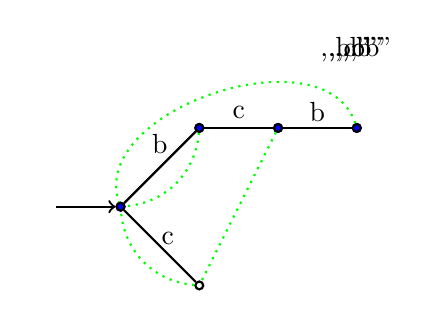
\begin{tikzpicture}
			\node[draw, circle, thick, white] (0) at (-1, 0) {};
			\onslide<all:6, 7> { \node at (3, 2) {,,bcb''}; }
			\onslide<all:8> { \node at (3, 2)     {,,cb''}; }
			\onslide<all:9> { \node at (3, 2)      {,,b''}; }
			\onslide<all:10-11> { \node at (3, 2)   {,,''}; }

			\onslide<all:7> { \node[draw, circle, fill, blue, thick, inner sep = 1.0pt] at (0, 0) {}; }
			\onslide<all:8> { \node[draw, circle, fill, blue, thick, inner sep = 1.0pt] at (1, 1) {}; }
			\onslide<all:9> { \node[draw, circle, fill, blue, thick, inner sep = 1.0pt] at (2, 1) {}; }
			\onslide<all:10> { \node[draw, circle, fill, blue, thick, inner sep = 1.0pt] at (3, 1) {}; }

			\node[draw, circle, thick, inner sep = 1.0pt] (1) at (0, 0) {};
			\node[draw, circle, thick, inner sep = 1.0pt] (2) at (1, 1) {};
			\node[draw, circle, thick, inner sep = 1.0pt] (3) at (2, 1) {};
			\node[draw, circle, thick, inner sep = 1.0pt] (4) at (3, 1) {};
			\node[draw, circle, thick, inner sep = 1.0pt] (5) at (1, -1) {};

			\path[draw, thick, ->] (0) -- (1);
			\path[draw, thick] (1) -- (2);
			\path[draw, thick] (2) -- (3);
			\path[draw, thick] (3) -- (4);
			\path[draw, thick] (1) -- (5);
			\path[draw, thick, green, dotted] (2) edge[bend left = 40] node {} (1);
			\path[draw, thick, green, dotted] (3) -- (5);
			%\path[draw, thick, green, dotted] (4) -- (6);
			\path[draw, thick, green, dotted] (4) edge[bend right = 90] node {} (1);
			\path[draw, thick, green, dotted] (5) edge[bend left = 40] node {} (1);

			\node at (0.5, 0.8) {b};
			\node at (1.5, 1.2) {c};
			\node at (2.5, 1.2) {b};
			\node at (0.6, -0.4) {c};
        \end{tikzpicture}
        \item<12-> To keep the complexity in check we again use dynamic programming.
        \item<13-> We add the concatenated links into the tree, calling them \emph{exit links}.
    \end{itemize}
\end{frame}

\begin{frame}[plain]{Speed}
	\begin{itemize}
        \item Let us assume the strings in $p$ appear $k$ times in $s$.
        \item Then the time complexity is $\mathcal{O}(|s| + |\Sigma| \cdot |p| + k)$
        \item If we only want the number of matches, the implementation can be modified accordingly and then the complexity is $\mathcal{O}(|s| + |\Sigma| \cdot |p|)$.
        \item Note that for a bounded alphabet, this second complexity is linear.
    \end{itemize}
\end{frame}

\begin{frame}[plain]{Implementation explanation}
	\begin{itemize}
        \item The implementation contains three helper functions.
        \item The first is \texttt{trie\_step(...)} which is used to move around the state machine.
        \item The second is \texttt{trie\_suffix(...)} which is used to find suffix links.
        \item The third is \texttt{trie\_exit(...)} which is used to find exit links.
        \item All these functions are recursive and memoized.
    \end{itemize}
\end{frame}

\begin{frame}[plain,fragile]{Aho nodes}
    \scriptsize
    \begin{minted}{cpp}
#define ALPHABET 128
// Helper function to get index of letter
int val(char c) { return c; }
struct listnode {
    // n is index of next node, v is value of this node
    int v, n;
    listnode(int _v, int _n) : v(_v), n(_n) { }
};
struct trienode {
    // l is the index of the pattern that ends here or -1 if none
    // e is the exit link index, d is the suffix link index
    // p is the parent index
    // c is the character of the incoming edge
    // t is the transition table of the trie node
    int t[ALPHABET], l, e, p, c, d;
    trienode(int _p, int _c) :
        l(-1), e(-1), p(_p), c(_c), d(-1) {
        memset(t, -1, sizeof(t));
    }
};
    \end{minted}
\end{frame}

\begin{frame}[plain,fragile]{Aho trie}
    \tiny
    \begin{multicols}{2}
    \begin{minted}{cpp}
struct trie { 
    // r is the index of the root
    int r;
    vector<trienode> m;
    vector<listnode> w;

    trie() {
        m = vector<trienode>();
        w = vector<listnode>();
        r = trie_node(-1, -1);
    }

    int list_node(int v, int n) {
        w.push_back(listnode(v, n));
        return w.size() - 1;
    }
    int trie_node(int p, int c) {
        m.push_back(trienode(p, c));
        return m.size() - 1;
    }

    void trie_insert(string &s, int x) {
        int h, i = 0;
        for(h = r; i < s.size(); h = m[h].t[val(s[i])], i++)
            if(m[h].t[val(s[i])] == -1)
                m[h].t[val(s[i])] = trie_node(h, val(s[i]));
        m[h].l = list_node(x, m[h].l);
    }
    \end{minted}
    \columnbreak
    \begin{minted}{cpp}
    int trie_suffix(int h) {
        if(m[h].d != -1) return m[h].d;
        if(h == r || m[h].p == r) return m[h].d = r;
        return m[h].d = 
            trie_step(trie_suffix(m[h].p), m[h].c);
    }

    int trie_step(int h, int c) {
        if(m[h].t[c] != -1) return m[h].t[c];
        return m[h].t[c] = h == r ? r :
            trie_step(trie_suffix(h), c);
    }

    int trie_exit(int h) {
        if(m[h].e != -1) return m[h].e;
        if(h == 0 || m[h].l != -1) return m[h].e = h;
        return m[h].e = trie_exit(trie_suffix(h));
    }
};
    \end{minted}
    \end{multicols}
\end{frame}

\begin{frame}[plain,fragile]{Aho implementation}
    \vspace{-25pt}
    \scriptsize
    \begin{minted}{cpp}
int aho_corasick(string &s, vector<string> &p) {
    trie t; int h, i, j, k, w, m = p.size(), l[m];
    for(i = 0; i < m; i++) l[i] = p[i].size();
    for(i = 0; i < m; i++) t.trie_insert(p[i], i);
    s.push_back('\0');
    for(i = 0, j = 0, h = t.r; j < s.size(); j++) {
        k = t.trie_exit(h);
        while(t.m[k].l != -1) {
            for(w = t.m[k].l; w != -1; w = t.w[w].n) {
                cout << p[t.w[w].v] << " found at index " << 
                    j - l[t.w[w].v] << '\n';
            }
            k = t.trie_exit(t.trie_suffix(k));
        }
        h = t.trie_step(h, val(s[j]));
    }
    return i;
}
    \end{minted}
\end{frame}

\begin{frame}{Suffix tries}
    \begin{itemize}
        \item Say we're dealing with some string $S$ of length $n$
        \vspace{10pt}
        \item Let's insert all suffixes of $S$ into a trie
        \vspace{10pt}
    \item $S$ = \texttt{banani}
        \begin{itemize}
    \item \texttt{insert(trie, "banani");}
    \item \texttt{insert(trie, "anani");}
    \item \texttt{insert(trie, "nani");}
    \item \texttt{insert(trie, "ani");}
    \item \texttt{insert(trie, "ni");}
    \item \texttt{insert(trie, "i");}
        \end{itemize}
    \end{itemize}
\end{frame}


\begin{frame}[fragile]{Suffix tries}

    \begin{center}
\begin{forest}
for tree={
    circle,
    fill=black!50,
    minimum size=12pt,inner sep=0pt, font=\tiny
  % circle,
  % black,
  % draw,
  % fill=blue!40,
}
  [{}
    [{}, edge label={node [midway, above left] {B}}
      [{}, edge label={node [midway, right] {A}}
        [{}, edge label={node [midway, right] {N}}
          [,phantom]
          [{}, edge label={node [midway, left] {A}}
            [{}, edge label={node [midway, left] {N}}
                [{}, edge label={node [midway, left] {I}}, fill=black!80
                ]
                [,phantom]
            ]
            [,phantom]
          ]
          [,phantom]
        ]
        [,phantom]
      ]
      [,phantom]
    ]
    [{}, edge label={node [midway, below right] {I}}, fill=black!80
        [,phantom]
    ]
    [{}, edge label={node [midway, right] {N}}
        % [,phantom]
        [{}, edge label={node [midway, left] {I}}, fill=black!80
        ]
      [{}, edge label={node [midway, right] {A}}
        [,phantom]
        [{}, edge label={node [midway, right] {N}}
          [,phantom]
          [{}, edge label={node [midway, right] {I}}, fill=black!80
          ]
        ]
      ]
        [,phantom]
    ]
    [{}, edge label={node [midway, above right] {A}}
      [,phantom]
      [{}, edge label={node [midway, right] {N}}
          [{}, edge label={node [midway, left] {I}}, fill=black!80 ]
        [{}, edge label={node [midway, right] {A}}
          [,phantom]
          [{}, edge label={node [midway, right] {N}}
            [,phantom]
            [{}, edge label={node [midway, right] {I}}, fill=black!80
            ]
          ]
        ]
      ]
    ]
  ]
\end{forest}
\end{center}
\end{frame}

\begin{frame}{Suffix tries}
    \begin{itemize}
        \item There are a lot of cool things we can do with suffix tries
        \vspace{10pt}
        \item Example: String matching
        \vspace{5pt}
        \item If a string $T$ is a substring in $S$, then (obviously) it has to start at some suffix of $S$
        \item So we can simply look for $T$ in the suffix trie of $S$, ignoring whether the last node is an end node or not
        \vspace{5pt}
        \item This is just $O(m)$...
    \end{itemize}
\end{frame}

\begin{frame}[fragile]{Suffix tries}

    \begin{center}
\begin{forest}
for tree={
    circle,
    fill=black!50,
    minimum size=12pt,inner sep=0pt, font=\tiny
  % circle,
  % black,
  % draw,
  % fill=blue!40,
}
  [{}, fill=red!50
    [{}, edge label={node [midway, above left] {B}}
      [{}, edge label={node [midway, right] {A}}
        [{}, edge label={node [midway, right] {N}}
          [,phantom]
          [{}, edge label={node [midway, left] {A}}
            [{}, edge label={node [midway, left] {N}}
                [{}, edge label={node [midway, left] {I}}, fill=black!80
                ]
                [,phantom]
            ]
            [,phantom]
          ]
          [,phantom]
        ]
        [,phantom]
      ]
      [,phantom]
    ]
    [{}, edge label={node [midway, below right] {I}}, fill=black!80
        [,phantom]
    ]
    [{}, edge label={node [midway, right] {N}}, fill=red!50
        % [,phantom]
        [{}, edge label={node [midway, left] {I}}, fill=black!80
        ]
      [{}, edge label={node [midway, right] {A}}, fill=red!50
        [,phantom]
        [{}, edge label={node [midway, right] {N}}, fill=red!50
          [,phantom]
          [{}, edge label={node [midway, right] {I}}, fill=black!80
          ]
        ]
      ]
        [,phantom]
    ]
    [{}, edge label={node [midway, above right] {A}}
      [,phantom]
      [{}, edge label={node [midway, right] {N}}
          [{}, edge label={node [midway, left] {I}}, fill=black!80 ]
        [{}, edge label={node [midway, right] {A}}
          [,phantom]
          [{}, edge label={node [midway, right] {N}}
            [,phantom]
            [{}, edge label={node [midway, right] {I}}, fill=black!80
            ]
          ]
        ]
      ]
    ]
  ]
\end{forest}
\end{center}
\end{frame}

\begin{frame}{Suffix tries}
    \begin{itemize}
        \item String matching is fast if we have the suffix trie for $S$
            \vspace{10pt}
        \item But what is the time complexity of suffix trie construction?
        \item There are $n$ suffixes, and it takes $O(n)$ to insert each of them
        \item So $O(n^2)$, which is pretty slow
            \vspace{10pt}
        \item Can we do better?
        \item There can be up to $n^2$ nodes in the graph, so this is actually optimal...
    \end{itemize}
\end{frame}

\begin{frame}{Suffix trees}
    \begin{itemize}
        \item There exists a compressed version of a suffix trie, called a suffix tree
        \vspace{10pt}
    \item It can be constructed in $O(n)$, and has all the features that suffix tries have
    \item But the $O(n)$ construction algorithm is pretty complex, a big disadvantage for us
    \end{itemize}
\end{frame}

\begin{frame}{Suffix arrays}
    \begin{itemize}
        \item A variation of the previous structures
        \item Can do everything the other structures can do, with a small overhead
        \item Can be constructed pretty quickly with relatively simple code
    \end{itemize}
\end{frame}

\begin{frame}[fragile]{Suffix arrays}
    \begin{itemize}
        \item Take all the suffixes of $S$
    \end{itemize}
    \begin{minted}{cpp}
banani
anani
nani
ani
ni
i

    \end{minted}
    \begin{itemize}
        \item and sort them
    \end{itemize}
    \begin{minted}{cpp}

anani
ani
banani
i
nani
ni
    \end{minted}

\end{frame}

\begin{frame}[fragile]{Suffix arrays}
    \begin{itemize}
        \item We can use this array to do everything that suffix tries can do
            \vspace{10pt}
        \item Like string matching
    \end{itemize}
\end{frame}

\begin{frame}[fragile]{Suffix arrays}
    \begin{itemize}
\item Let's look for \texttt{nan}
\item<2-> The first letter in the string has to be \texttt{n}, so we can binary search for the range of strings starting with \texttt{n}
    \end{itemize}
    \vspace{10pt}
    \begin{minted}{cpp}

anani
ani
banani
i
nani
ni
    \end{minted}
\end{frame}

\begin{frame}[fragile]{Suffix arrays}
    \begin{itemize}
\item Let's look for \texttt{nan}
\item The first letter in the string has to be \texttt{n}, so we can binary search for the range of strings starting with \texttt{n}
    \end{itemize}
    \vspace{10pt}
    \begin{minted}{cpp}





nani
ni
    \end{minted}
\end{frame}

\begin{frame}[fragile]{Suffix arrays}
    \begin{itemize}
\item Let's look for \texttt{nan}
\item The second letter in the string has to be \texttt{a}, so we can binary search for the range of strings that have \texttt{a} as the second letter
    \end{itemize}
    \vspace{10pt}
    \begin{minted}{cpp}





nani
ni
    \end{minted}
\end{frame}

\begin{frame}[fragile]{Suffix arrays}
    \begin{itemize}
\item Let's look for \texttt{nan}
\item The second letter in the string has to be \texttt{a}, so we can binary search for the range of strings that have \texttt{a} as the second letter
    \end{itemize}
    \vspace{10pt}
    \begin{minted}{cpp}
nani
    \end{minted}
\end{frame}

\begin{frame}[fragile]{Suffix arrays}
    \begin{itemize}
\item Let's look for \texttt{nan}
\item The third letter in the string has to be \texttt{n}, so we can binary search for the range of strings that have \texttt{n} as the third letter
    \end{itemize}
    \vspace{10pt}
    \begin{minted}{cpp}
nani
    \end{minted}
\end{frame}

\begin{frame}[fragile]{Suffix arrays}
    \begin{itemize}
\item Let's look for \texttt{nan}
\item The third letter in the string has to be \texttt{n}, so we can binary search for the range of strings that have \texttt{n} as the third letter
    \end{itemize}
    \vspace{10pt}
    \begin{minted}{cpp}
nani
    \end{minted}
    \begin{itemize}
\item<2-> If there is at least one string left, we have a match
    \end{itemize}
\end{frame}

\begin{frame}{Suffix arrays}
    \begin{itemize}
        \item Time complexity?
            \vspace{5pt}
        \item For each letter in $T$, we do two binary searches on the $n$ suffixes to find the new range
        \item Time complexity is $O(m \times \log n)$
            \vspace{10pt}
        \item A bit slower than doing it with a suffix trie, but still not bad
    \end{itemize}
\end{frame}

\begin{frame}{Suffix arrays}
    \begin{itemize}
        \item But how do we construct a suffix array for a string?
            \vspace{10pt}
        \item A simple \texttt{sort(suffixes)} is $O(n^2\log(n))$, because comparing two suffixes is $O(n)$
        \item And we still have the same problem as with suffix tries, there are almost $n^2$ characters if we store all suffixes
    \end{itemize}
\end{frame}

\begin{frame}[fragile]{Suffix arrays}
    \begin{itemize}
        \item The second problem is easy to fix
        \item Just store the indices of the suffixes
    \end{itemize}
    \begin{minted}[fontsize=\footnotesize]{cpp}
anani
ani
banani
i
nani
ni
    \end{minted}
    \begin{itemize}
        \item becomes
    \end{itemize}
    \begin{minted}[fontsize=\footnotesize]{cpp}
1: anani
3: ani
0: banani
5: i
2: nani
4: ni
    \end{minted}
\end{frame}

\begin{frame}{Suffix arrays}
    \begin{itemize}
        \item What about the construction?
        \item In short, we
            \begin{itemize}
                \item sort all suffixes by only looking at the first letter
                \item sort all suffixes by only looking at the first 2 letters
                \item sort all suffixes by only looking at the first 4 letters
                \item sort all suffixes by only looking at the first 8 letters
                \item \ldots
                \item sort all suffixes by only looking at the first $2^i$ letters
                \item \ldots
            \end{itemize}
        \vspace{10pt}
    \item If we use an $O(n\log n)$ sorting algorithm, this is $O(n\log^2 n)$
    \item We can also use an $O(n)$ sorting algorithm, since all sorted values are between $0$ and $n$, bringing it down to $O(n \log n)$
    \end{itemize}
\end{frame}

\begin{frame}[fragile]{Suffix arrays}
    \begin{minted}[fontsize=\footnotesize]{cpp}
struct suffix_array {
    struct entry {
        pair<int, int> nr;
        int p;

        bool operator <(const entry &other) {
            return nr < other.nr;
        }
    };


    string s;
    int n;
    vector<vector<int> > P;
    vector<entry> L;
    vi idx;

    // constructor
};
\end{minted}
\end{frame}

\begin{frame}[fragile]{Suffix arrays}
    \begin{minted}[fontsize=\tiny]{cpp}
suffix_array(string _s) : s(_s), n(s.size()) {
    L = vector<entry>(n);
    P.push_back(vi(n));
    idx = vi(n);

    for (int i = 0; i < n; i++) {
        P[0][i] = s[i];
    }

    for (int stp = 1, cnt = 1; (cnt >> 1) < n; stp++, cnt <<= 1) {
        P.push_back(vi(n));
        for (int i = 0; i < n; i++) {
            L[i].p = i;
            L[i].nr = make_pair(P[stp - 1][i], i + cnt < n ? P[stp - 1][i + cnt] : -1);
        }

        sort(L.begin(), L.end());
        for (int i = 0; i < n; i++) {
            if (i > 0 && L[i].nr == L[i - 1].nr) {
                P[stp][L[i].p] = P[stp][L[i - 1].p];
            } else {
                P[stp][L[i].p] = i;
            }
        }
    }

    for (int i = 0; i < n; i++) {
        idx[P[P.size() - 1][i]] = i;
    }
}
\end{minted}
\end{frame}

\begin{frame}[fragile]{Suffix arrays}
    \begin{itemize}
        \item There is also one other useful operation on suffix arrays
        \item Finding the longest common prefix (lcp) of two suffixes of $S$
    \end{itemize}

    \begin{minted}[fontsize=\footnotesize]{cpp}
1: anani
3: ani
0: banani
5: i
2: nani
4: ni
    \end{minted}

    \begin{itemize}
\item \texttt{lcp(1,3) = 2}
\item \texttt{lcp(2,1) = 0}
    \vspace{10pt}
\item This function can be implemented in $O(\log n)$ by using intermediate results from the suffix array construction
    \end{itemize}
\end{frame}

\begin{frame}[fragile]{Suffix arrays}
    \begin{minted}[fontsize=\footnotesize]{cpp}
int lcp(int x, int y) {
    int res = 0;
    if (x == y) return n - x;
    for (int k = P.size() - 1; k >= 0 && x < n && y < n; k--) {
        if (P[k][x] == P[k][y]) {
            x += 1 << k;
            y += 1 << k;
            res += 1 << k;
        }
    }
    return res;
}
\end{minted}
\end{frame}

\begin{frame}{Longest common substring}
    \begin{itemize}
        \item Given two strings $S$ and $T$, find their longest common substring
            \vspace{10pt}
        \item \texttt{S = banani}
        \item \texttt{T = kanina}
            \vspace{10pt}
        \item Their longest common substring is \texttt{ani}
            \vspace{20pt}
        \item \textit{see example}
    \end{itemize}
\end{frame}

\end{document}


